\documentclass[a4paper]{amsart}

\usepackage{color}
\usepackage[colorlinks=true, citecolor=red]{hyperref}  %needs to come before amsrefs package to work with \cite{}*{}
\usepackage{amssymb,latexsym}
\usepackage[alphabetic]{amsrefs}
\usepackage[mathscr]{eucal}
\usepackage{pdfsync}
\usepackage{graphicx}
\usepackage{epstopdf}
\DeclareGraphicsRule{.tif}{png}{.png}{`convert #1 `dirname #1`/`basename #1 .tif`.png}
\usepackage[all]{xy}
\usepackage{titletoc}
%\usepackage{showkeys}  %options notref  notcite 

%\input{rgb.tex}

\CompileMatrices

\theoremstyle{plain}
\newtheorem{theorem}{Theorem}[section]
\newtheorem{lemma}[theorem]{Lemma}
\newtheorem{proposition}[theorem]{Proposition}
\newtheorem{corollary}[theorem]{Corollary}

\theoremstyle{definition}
\newtheorem{definition}[theorem]{Definition}%[section]
\newtheorem{constr}[theorem]{Construction}
\newtheorem{notation}[theorem]{Notation}


\theoremstyle{remark}
\newtheorem{defn}[theorem]{Definition} 
\newtheorem{example}[theorem]{Example}
\newtheorem{remark}[theorem]{Remark}
\newtheorem{discussion}[theorem]{Discussion}

%\numberwithin{equation}{section}

%\newcommand{\abs}[1]{\lvert#1\rvert}

\DeclareMathOperator{\Lip}{Lip}
\DeclareMathOperator{\dist}{dist}
\DeclareMathOperator{\expected}{\mathbb{E}}
\DeclareMathOperator{\prb}{Prob}
\DeclareMathOperator{\spt}{spt}
\DeclareMathOperator{\lap}{\Delta}
\DeclareMathOperator{\Tr}{Tr}

\raggedbottom

\addtolength{\textwidth}{2cm}
\addtolength{\oddsidemargin}{-1cm}
\addtolength{\evensidemargin}{-1cm} 
\addtolength{\topmargin}{-1cm} 
\addtolength{\textheight}{2cm}

\setcounter{tocdepth}{3}



%%% BEGIN DOCUMENT
\begin{document}

\title{Avoiding Furstenberg Kesten}  
\author{Notes by John E.\ Hutchinson}
\date{\today}

%\begin{abstract} 
%\end{abstract}

\maketitle

\tableofcontents


%%%%%%%%%%%%%%%%%%%%%%%%%%%%%%%%
%%%%%%%%%%%%%%%%%%%%%%%%%%%%%%%%
%%%%%%%%%%%%%%%%%%%%%%%%%%%%%%%%
%%%%%%%%%%%%%%%%%%%%%%%%%%%%%%%%


\section{\textbf{11/10/10 $ V $-Variability via Types}}
We show how $ V $-variable trees can be constructed by using ``types'' instead  of working with $ V $-tuples of sets.


\medskip (We follow the usual notation and conventions for finite sequences involving truncation, concatenation, length and initial segment.)

\medskip
In the following   fix $ V \in \mathbb{N} $ and fix a family $ \boldsymbol{F} $ of IFSs.

\medskip 
Consider finitely branching trees $ T $ with a single root node and no terminating branches.  In the applications each node will have at least two children.  More precisely:

\begin{definition} A \emph{tree} $ T $ is a subset of the set of finite sequences of elements from $ \mathbb{N} $.  
\begin{enumerate}
\item If $ \emptyset $ is the empty sequence then $ \emptyset \in T $. 
\item Suppose  $ \boldsymbol{i} \in T $. Then  $  \boldsymbol{i} j \in T \text{ iff }  1 \leq j \leq N $, for some $ N\geq 2  $ depending on $ \boldsymbol{i} $. We call $ N $ the \emph{branching number} at $ \boldsymbol{i} $.
\item If $ \boldsymbol{i} \in T $ then $ \boldsymbol{j} \in T $ for any $ \boldsymbol{j} \preccurlyeq \boldsymbol{i} $.
\end{enumerate} 
\end{definition} 

Then $ \emptyset $ is called the \emph{root node}, the nodes  $  \boldsymbol{i} j $  in (2)  are the \emph{children} of $ \boldsymbol{i} $ for $ 1\leq j \leq N $, and the (unique) \emph{parent} of $ \boldsymbol{i} $ is  $ \boldsymbol{i} | (k-1) $ where $ k = | \boldsymbol{i} | $ is the length of $ \boldsymbol{i} $.

\bigskip 
\begin{definition} A \emph{$ V $-variable tree} $ T $ is a certain kind of \emph{labelled} tree.  
Each node $ \boldsymbol{i}\in T$ is assigned a pair $ ( \tau ^ { \boldsymbol{i} } , F^{ \boldsymbol{i} })$   where $  \tau ^ { \boldsymbol{i} }\in \{ 1,\dots, V\} $ is called the \emph{type  assigned to $ \boldsymbol{i} $}, and $ F^ { \boldsymbol{i}} \in \boldsymbol{F} $  is called \emph{the IFS assigned to $ \boldsymbol{i} $}.  

The branching number $ N^{ \boldsymbol{i} } $ at $ \boldsymbol{i} $ is the cardinality of $ F^ { \boldsymbol{i} }= (f^{ \boldsymbol{i} }_1,\dots , f^{ \boldsymbol{i} }_N)$. The function $ f^{ \boldsymbol{i} }_k $ corresponds to  the $ k$th  edge  from $ \boldsymbol{i} $, joining $ \boldsymbol{i} $ to $  \boldsymbol{i} k $.

If two nodes $ \boldsymbol{i} $ and $  \boldsymbol{j} $ at the same level have the same type   they are assigned the same IFS, and their  corresponding  children are assigned corresponding types.  

Summarising:
\begin{equation} \label{vpr} 
| \boldsymbol{i} | = | \boldsymbol{j} |  \text{ \& } 
                   \tau ^ { \boldsymbol{i} } =  \tau ^ { \boldsymbol{j} }
\Longrightarrow 
\begin{cases}   F ^ { \boldsymbol{i} }= F ^ { \boldsymbol{j} } & \\
                      N ^ { \boldsymbol{i} }= N ^ { \boldsymbol{j} } =: N & \\
                       \tau ^ { \boldsymbol{i}k}  =  \tau ^ { \boldsymbol{j}k } &\text{if } 1 \leq k \leq N  
                       \end{cases}. 
\end{equation} 

The \emph{set of $ V $ -variable trees}  is denoted by $ \mathcal{T} =  \mathcal{T} _V $.
 \end{definition} 
 
 In order to construct $ V  $-variable trees it is convenient to introduce the following notion.

\begin{definition}  We say $ \widetilde{F} = (F, \tau_1,\dots, \tau_N) $ is an \emph{IFS/type vector}  if $ F \in \boldsymbol{F} $, $ N $ is the cardinality of $ F $ and $ \tau_1,\dots, \tau_N \in \{1,\dots, V\}  $.  The \emph{set of IFS/type vectors} is denoted by  $ \widetilde{ \boldsymbol{F} } $.
\end{definition} 

\medskip The informal idea in the following construction is as follows.

Initially one assigns a type to the root node, and w.l.o.g.\ the type is 1.

At stage (1) in the construction an IFS/type vector $ \widetilde{F}(v) $ is selected  for each   $ v \in \{1,\dots, V \} $. Using $  \widetilde{F}(1) $ an IFS is assigned to the root node and a type to each of its children, the level 1 nodes.%
\footnote{The $ \widetilde{F}(v) $ selected at stage 1  for $ v \neq 1 $ are not used in the construction, and are included only for consistency with the construction at later stages.}

At stage (2)  an IFS/type vector $ \widetilde{F}(v) $ is selected  for each   $ v \in \{1,\dots, V \} $. For each level 1 node, if $ v $ is the type of the node, then via 
 $  \widetilde{F}(v) $  an IFS is assigned to the node and a type is assigned to each of its children.  In particular a type is assigned to every level 2 node. 

At stage (n)  an IFS/type vector $ \widetilde{F}(v) $ is selected  for each   $ v \in \{1,\dots, V \} $. For each level $ n-1 $  node, if $ v $ is the type of the node, then via 
 $  \widetilde{F}(v) $  an IFS is assigned to the node and a type is assigned to each of its children.   In particular a type is assigned to every level $ n $  node. 
                       
\medskip
\begin{constr}\label{constrV}
A type $ \tau ^ \emptyset \in \{1,\dots, V \} $ is assigned to the root node $ \emptyset $.
W.l.o.g.\  let $ \tau ^ \emptyset =1 $.  

The tree is constructed  by recursion  as follows.
\begin{enumerate}
\item Select  $ \widetilde{F}(v) \in \widetilde{ \boldsymbol{F} }$  for $ v =1,\dots, V $.  (Note that the type 1 has already been assigned to the level 0 node.)
Assign an IFS and a branching number to the level 0 node $ \emptyset $,  and a type to each level 1 node $ k $, by
\[
F^{\emptyset}= F,\ N^{\emptyset}=N, \ \tau^k = \tau_k, \quad  \text{where } F(1)  = (F,\tau_1,\dots, \tau_N ) \text{ and  } 1 \leq k \leq  N .
\]

\item  Select  $ \widetilde{F}(v) \in \widetilde{ \boldsymbol{F} }$  for $ v =1,\dots, V $.  (Note that a type   has already been assigned to each level 1 node.)
Assign an IFS and a branching number to each level 1 node $ \ell $, and a type to each level 2 node
$ \ell k $, by setting
\[
F^\ell = F, \ N^\ell =N, \ \tau^{ \ell k} = \tau_k, \quad \text{where } F(\tau^\ell)  = (F,\tau_1,\dots, \tau_N ) \text{ and  } 1 \leq k \leq  N .
\]

\item[($  n $)]  Select $ \widetilde{F}(v) \in \widetilde{ \boldsymbol{F} }$  for $ v =1,\dots, V $.  (Note that a type   has already been assigned to each level $ n-1 $  node.)
Assign an IFS and a branching number to each level $ n- 1$  node, and a type to each level $ n $ node, by
\[
F^{ \boldsymbol{i} }  = F, \ N^{ \boldsymbol{i} }  =N, \ \tau^{  \boldsymbol{i} \ell} = \tau_k \quad \text{where } F(\tau^{ \boldsymbol{i} } )  = (F,\tau_1,\dots, \tau_N ) \text{ and  } 1 \leq k \leq  N .
\]
\end{enumerate} 
\end{constr}


%\bigskip *** Following is OLD version ***
%\begin{itemize} 
%\item[(1)] 
%\begin{itemize} 
%\item[(a)] An IFS from $ \boldsymbol{F} $ is assigned to the type   at level 0. Equivalently, this assigns an IFS $ F^\emptyset $   to the  level 0 node. 
%The branching number at $ \emptyset $ is  the cardinality of $F^\emptyset $. 
%
%\item[(b)] To each level 1 node $ k $ is assigned a type $ \tau ^k \in \{1,\dots,V\} $. 
%\end{itemize} 
%
%\item[(2)]  
%\begin{itemize} 
%\item[(a)] An IFS from $ \boldsymbol{F} $ is assigned to each type at level 1.  This assigns an IFS $ F^k $ to each level 1 node $ k $. The branching number at $ k $ is  the cardinality of $  F^k $.
% (Thus level 1 nodes of the same type are assigned the same IFS and have the same branching number.)
%
%\item[(b)] To each level 2 node $ k \ell $ is assigned a type $ \tau ^{k \ell} \in \{1,\dots,V\} $ in such a way that corresponding nodes with the same parent type will themselves have the same type. 
%\end{itemize} 
%\item[($ n$)]  
%\begin{itemize} 
%\item[(a)] An IFS from $ \boldsymbol{F} $ is assigned to each type at level $ n- 1$.  This assigns an IFS $ F^{\boldsymbol{i} } $ to each level $ n-1 $  node $ \boldsymbol{i}  $. The branching number at $ \boldsymbol{i}  $ is  the cardinality of $  F^{ \boldsymbol{i} }  $.
% (Thus level $ n-1$ nodes of the same type are assigned the same IFS and have the same branching number.)
%
%\item[(b)] To each level $ n $  node $ \boldsymbol{j} $ is assigned a type $ \tau ^{ \boldsymbol{j} } \in \{1,\dots,V\} $ in such a way that corresponding nodes with the same parent type will themselves have the same type. 
%\end{itemize} 
%
%\end{itemize} 
% 
%
%It is easy to see by induction that any labelled tree constructed in this manner satisfies \eqref{vpr}, and that any labelled tree satisfying  \eqref{vpr} can be so constructed.
%
%*** end of OLD version ***

\begin{notation}  The particular tree $ T $ will usually be understood from context.

We   use the convention that quantities defined from the IFS or the type at the node $ \boldsymbol{i} \in T   $ are denoted with   \emph{superscript} $ \boldsymbol{i} $.  For example, the type, the IFS and the branching number  at $ \boldsymbol{i}  $ are denoted by $ \tau^{\boldsymbol{i} } $, $ F^{ \boldsymbol{i} } $ and $ N^{ \boldsymbol{i} } $  respectively.
Similarly we write $  F^{ \boldsymbol{i} } = 
    \big( f^{ \boldsymbol{i}}_1  , \dots, f^{ \boldsymbol{i}}_{N^{ \boldsymbol{i} } }\big) $.  
    
We associate the function $  f^{ \boldsymbol{i}}_j $ to the $ j $th  \emph{edge} with initial node $ \boldsymbol{i} $ and hence with terminal node~$ \boldsymbol{i} j $.   Similarly, let $ \ell^{ \boldsymbol{i} }_j $ be the Lipschitz constant of    $ f^{ \boldsymbol{i} }_j $.   
    
  Other quantities associated to the node $ \boldsymbol{i} $ will depend not only on $ (\tau^ { \boldsymbol{i}  } , F^{ \boldsymbol{i} }) $ but will be obtained by multiplying or composing certain quantities or functions along the sequence of edges connecting $ \emptyset $ to $ \boldsymbol{i} $.  We will usually use a \emph{subscript} $ \boldsymbol{i} $ in this case.   
     In particular, we multiply the Lipschitz constants and compose the contraction maps associated with the edges joining $ \emptyset $ to $ \boldsymbol{i} $ to obtain the following with   $ k = | \boldsymbol{i} | $:
    \begin{align*}
    f_{\boldsymbol{i} } &= f^{ \emptyset}_{i_1} \circ f^{ i_1}_{i_2} \circ f^{ i_1 i_2}_{i_3}\circ 
                                         \ldots \circ f^{ i_1 i_2\dots i_{k-1}}_{i_k}, \\
    \ell_{\boldsymbol{i} } &= \ell^{ \emptyset}_{i_1} \cdot \ell^{ i_1}_{i_2} \cdot \ell^{ i_1 i_2}_{i_3}\cdot 
                                         \ldots \cdot \ell^{ i_1 i_2\dots i_{k-1}}_{i_k}.
\end{align*} 
\end{notation}                                         
    
    


%%%%%%%%%%%%%%%%%%%%%%%%%%%%%%%%%
%%%%%%%%%%%%%%%%%%%%%%%%%%%%%%%%%
\section{\textbf{The Probability Distribution on the Set of $ V $-Variable Trees}}

Fix a probability distribution $ P $ on $ \boldsymbol{F} $.  

 
\begin{definition} The probability distribution on $ \widetilde{ \boldsymbol{F} } $ is the distribution  of the random vector 
$ 
\widetilde{F} =  (F  , v_1,\dots, v_N  )   $, 
 where 
 $ F $ is a random IFS with distribution $ P $, $ N $ is the cardinality of $ F $  and $ v_1,v_2,\dots $ are iid random variables uniformly distributed on $ \{ 1,\dots, V \} $ independent of $ F $.

We   denote this probability distribution on $ \widetilde{ \boldsymbol{F} } $ also by $ P $. 
\end{definition} 

 

The $ V $-variable tree $ T $ in Construction~\ref{constrV} is uniquely  determined 
by the sequence 
\[
\mathcal{E} _1, \mathcal{E} _2, \dots, \mathcal{E} _n , \dots ,
\]
where $ \mathcal{E} _n $ is the $ V $-tuple of  IFS/type vectors selected at level $ n $.
This leads to the following definition.

\begin{definition} The \emph{distribution $ P = P_V $ on the set $ \mathcal{T} _V $} of $ V  $-variable trees  is obtained by selecting each  of the $ V $ 
IFS/type vectors at stage $ n $ in Construction~\ref{constrV}  according to the distribution $ P $ on $ \widetilde{ \boldsymbol{F} } $, in an iid manner and independent of the IFS/type vectors at all other stages. 
\end{definition} 

\begin{notation} \label{notsup} Realisations of a random $ V $-variable tree may be denoted by  $ T^\omega $, but usually the $ \omega $ is suppressed.

In situations where more than one tree is being considered, an appropriate superscript will again be used, with parentheses if needed for clarity.  
For example, if $ T $ is a given tree and $ \boldsymbol{i} \in T $ then the subtree rooted at $ \boldsymbol{i} $ is denoted $ T^{ \boldsymbol{i} } = T^{ (\boldsymbol{i}) }$.  In particular, $ T^{(\emptyset)} = T $. If $ \boldsymbol{j} $ is a node of $ T^{ (\boldsymbol{i}) } $ then the corresponding node of  $ T $ is $ \boldsymbol{i} \boldsymbol{j} $.  Similarly, $ F^{ (\boldsymbol{i}), \boldsymbol{j} } = F^{ \boldsymbol{i}   \boldsymbol{j} } = F^{ (\emptyset), \boldsymbol{i}   \boldsymbol{j} } $; that is, the IFS at node $ \boldsymbol{j} $ of the subtree $ T^{ (\boldsymbol{i}) } $  is the same as the IFS at node $ \boldsymbol{i} \boldsymbol{j} $ of the tree $ T $, and the tree $ T $  is just the tree $  T^{ (\emptyset)} $. Similar notation applies to other quantities besides $ F $.

If $ n(1) < n(2) < \cdots $ is the sequence of necks for $ T $, then $ T^{ \boldsymbol{i} }= T^{ \boldsymbol{j} } $ if $ | \boldsymbol{i} | = | \boldsymbol{j} | = n(k) $ for some $ k $.  In this case we define   $ T^{(k)} = T^{ \boldsymbol{i} }    $ and    $ F^{(k), \boldsymbol{j} } =  F^{ (\boldsymbol{i}),   \boldsymbol{j} }  =  F^{ \boldsymbol{i}   \boldsymbol{j} } $ for  any  $ \boldsymbol{i} $ with $ | \boldsymbol{i} |= n(k) $.  Again, similar notation applies  to other quantities besides $ F $.
 \end{notation}

\bigskip
%*** Following is OLD version ***
%We first give a slightly informal description.
%
%\medskip  \begin{itemize} 
%\item[(0)] The type $ \tau ^\emptyset \in \{1,\dots, V\} $ is chosen according to the uniform distribution.  
%
%\item[(1)] 
%\begin{itemize} 
%\item[(a)] The IFS $ F^\emptyset $ is chosen according to $ P $.  In particular this determines the branching number $ N^\emptyset $.
%\item[(b)] Each type  $ \tau^k $ for $ 1 \leq k \leq N^\emptyset $ is chosen from $ \{ 1,\dots,V\} $ in an iid manner according to the uniform distribution and  independently  of $ \tau^\emptyset $ and $ F^\emptyset $. (Of course, the \emph{number} of nodes at level 1 depends on $ F^\emptyset $)
%\end{itemize} 
%
%\item[(2)] 
%\begin{itemize} 
%\item[(a)] For each type $ \tau \in \{1,\dots,V\} $ there is chosen an IFS according to $ \boldsymbol{F} $ in an iid manner independently of any choices already made.   Using the type assigned at the previous step (1)(b) to the node $ k $    this assigns an IFS $ F^k $ to $ k $ and determines the branching number $ N^k $ at $ k $.
%(Hence level 1 nodes of the same type are assigned the same IFS and have the same branching number.)
%
%\item[(b)]  Each type $ \tau^{kl} $ where  $  1 \leq k \leq N^\emptyset $ and $    1 \leq \ell \leq N^k $
%is chosen in an iid manner according to the uniform distribution and  independently  of any choices already made.
%\end{itemize} 
%
%\item[($ n $)] 
%\begin{itemize} 
%\item[(a)] For each type $ \tau \in \{1,\dots,V\} $ there is chosen an IFS according to $ \boldsymbol{F} $ in an iid manner independently of any choices already made.   Using the type assigned at the previous step ($ n-1$)(b) to the level $ n-1 $ node $ \boldsymbol{i}  $    this assigns an IFS $ F^{ \boldsymbol{i} }  $ to $ \boldsymbol{i}  $ and determines the branching number $ N^{ \boldsymbol{i} } $ at $ \boldsymbol{i}  $.
%(Hence level $ n-1 $  nodes of the same type are assigned the same IFS and have the same branching number.)
%
%\item[(b)]  Each type $ \tau^{\boldsymbol{i} l} $ where  $ \boldsymbol{i} $ is a level $ n-1 $ node, $  1 \leq k \leq N^{ \boldsymbol{i} } $ and $    1 \leq \ell \leq N^ { \boldsymbol{i} } $,
%is chosen in an iid manner according to the uniform distribution and  independently  of any choices already made.
%\end{itemize} 
%\end{itemize} 
%
%
%In the preceding we   described the probability distribution $ P_V$  on the space $ \mathcal{T} _V $ of $ V $-variable trees.  Although there is a high degree of independency involved, this is a little obscured because the number of nodes at each level depends on the choice of type and IFS at previous nodes.
%
%*** End of OLD version ***
%
%%%%%%%%%%%%%%%%%%%%%%%%%%%%%%%%%
%%%%%%%%%%%%%%%%%%%%%%%%%%%%%%%%%
\section{\textbf{Avoiding Furstenberg Kesten}}


Assume
\begin{equation} \label{} 
\begin{aligned} 
N_{\max} &:= \sup \big\{N : F = (f_1,\dots, f_N) \in \boldsymbol{F}  \big\} < \infty \\
\ell_{\max} &:= \sup \big\{ \Lip f_j : F = (f_1,\dots, f_N) \in \boldsymbol{F}   ,\ 1\leq i \leq N\big\} < 1.
\end{aligned} 
\end{equation} 

Recall that the sequence of necks follows a geometric distribution.  Let $ q $ be the probability of a  neck occurring at any particular level.  

\medskip Assume the $ V $-variable random tree $ T $ has distribution  $ P_V $.  Let $ T = T^ \omega $ be a realisation.

\medskip For $ \boldsymbol{i} \in T $  and $ | \boldsymbol{i} | = n $   define
\[
r_{ \boldsymbol{i} } =   r_{i_1}^\emptyset \cdot r_{i_2}^{i_1} \cdot   r_{i_3}^{i_1i_2} \cdot \ldots  
          \cdot r_{ i_n }^{ i_1\dots i_{n-1} }  ,
\]
where $ r_k^{ \boldsymbol{i} } = (\ell _k^{ \boldsymbol{i} } ) ^{ \alpha } = (\Lip f _k^{ \boldsymbol{i} } ) ^{ \alpha } $  and $ \alpha > 0 $. Let $ r_{\max} = \ell_{\max}^ \alpha $.

\begin{theorem} The expected exponential growth rate of  $  \sum_{ | \boldsymbol{i} | = n } r_{ \boldsymbol{i} }$, namely
\begin{equation} \label{} 
 \lim_{n\to \infty} \frac{1}{n}\expected \log \sum_{ | \boldsymbol{i} | = n } r_{ \boldsymbol{i} }
=: \gamma =: \gamma ( \alpha ) ,
\end{equation} 
exists and is finite. Moreover,
\begin{equation} \label{pwl} 
 \lim_{n\to \infty} \frac{1}{n} \log \sum_{ | \boldsymbol{i} | = n } r_{ \boldsymbol{i} }
  = \gamma \text{ a.s.}
\end{equation} 
Also, one has  the formula 
\begin{equation} \label{} 
\gamma = q\,  \expected \log \sum_{ | \boldsymbol{i} | = n(1) } r_{ \boldsymbol{i} },
\end{equation} 

\end{theorem} 

\begin{proof}  We begin by considering limits through the sequence of necks:
\begin{equation} \label{ltn} 
\lim_{k\to \infty} \frac{1}{n(k)} \log \sum_{ | \boldsymbol{i} | = n(k) } r_{ \boldsymbol{i} } .
\end{equation} 

Then
{\allowdisplaybreaks 
\begin{align} 
&\sum_{\boldsymbol{i} \in T, | \boldsymbol{i} | = n(k) } r_{ \boldsymbol{i} }   \notag \\
& =
\sum_{\boldsymbol{i} \in T, | \boldsymbol{i} | = n(k) }
  r_{i_1}^\emptyset \cdot r_{i_2}^{i_1} \cdot   r_{i_3}^{i_1i_2} \cdot \ldots  
          \cdot r_{ i_{n(k)} }^{ \boldsymbol{i} | ( n(k) - 1) }  \notag \\
 &= 
  \sum_{\boldsymbol{i} \in T, | \boldsymbol{i} | = n(k)  }
\bigg\{ \left(    r_{i_1}^\emptyset \cdot r_{i_2}^{i_1}\cdot r_{i_3}^{i_1i_2} \cdot
                            \ldots \cdot r_{ i_{n(1)} }^{ \boldsymbol{i} | ( n(1) - 1) }    \right)  \notag\\
&\qquad  \qquad \qquad \quad  \cdot    \left(    r_{i_{n(1)+1}}^{ \boldsymbol{i} | n(1)}  
               \cdot  r_{ i_{n(1)+2} }^{ \boldsymbol{i} | n(1)+1 } 
                     \cdot \ldots \cdot r_{ i_{n(2)} }^{ \boldsymbol{i} | ( n(2) - 1) } \right) \cdot \ldots \notag\\
& \qquad  \qquad \qquad  \quad  \cdot   \left(    r_{i_{n(k-1)+1}}^{ \boldsymbol{i} | n(k-1)}  
                      \cdot  r_{ i_{n(k-1)+2} }^{ \boldsymbol{i} | n(k-1)+1 } 
                     \cdot \ldots \cdot r_{ i_{n(k)} }^{ \boldsymbol{i} | ( n(k) - 1) } \right)  \bigg\}  
          \notag    \\
%&=\sum_{| \boldsymbol{i} | = n(k)  } 
%\bigg\{  \left(  r_{i_1}^{(0),\emptyset} \cdot r_{i_2}^{(0),i_1}\cdot r_{i_3}^{(0),i_1i_2} \cdot
%                            \ldots \cdot r_{ i_{n(1)} }^{(0), \boldsymbol{i} | ( n(1) - 1) }    \right) \\
%& \qquad  \qquad \quad   \cdot  \left(  r_{i_1}^{(1),\emptyset} \cdot r_{i_2}^{(1),i_1}\cdot r_{i_3}^{(1),i_1i_2} \cdot  \ldots \cdot r_{ i_{n(2) - n(1)} }^{(1), \boldsymbol{i} | ( n(2) - n(1) -1) } \right) \cdot \ldots \\
% &  \qquad  \qquad \quad \cdot  \left(  r_{i_1}^{(k-1),\emptyset} \cdot r_{i_2}^{(k-1),i_1}\cdot r_{i_3}^{(k-1),i_1i_2} \cdot
% \ldots \cdot r_{ i_{n(2) - n(1)} }^{(k-1), \boldsymbol{i} | ( n(2) - n(1) -1) } \right)\ \bigg\} 
%              \\
&=  
   \Bigg( \sum_{\boldsymbol{i} \in T^{(0)}, | \boldsymbol{i} | = n(1) }
         r_{i_1}^{(0),\emptyset} \cdot r_{i_2}^{(0),i_1}\cdot r_{i_3}^{(0),i_1i_2} \cdot
                            \ldots \cdot r_{ i_{n(1)} }^{(0), \boldsymbol{i} | ( n(1) - 1) }  \Bigg)  \notag \\
 &\quad   \cdot                               
         \Bigg( \sum_{\boldsymbol{i} \in T^{(1)}, | \boldsymbol{i} | = n(2)-n(1) }
         r_{i_1}^{(1),\emptyset} \cdot r_{i_2}^{(1),i_1}\cdot r_{i_3}^{(1),i_1i_2} \cdot
                            \ldots \cdot r_{ i_{n(2)-n(1)} }^{(1), \boldsymbol{i} | ( n(2) -n(1) - 1) }  \Bigg) 
                                         \cdot \ldots \notag\\
& \quad  \cdot                               
         \Bigg( \sum_{\boldsymbol{i} \in T^{(k-1)}, | \boldsymbol{i} | = n(k)-n(k-1) }
         r_{i_1}^{(k-1),\emptyset} \cdot r_{i_2}^{(k-1),i_1}\cdot r_{i_3}^{(k-1),i_1i_2} \cdot
                           \ldots \cdot r_{ i_{n(k)-n(k-1)} }^{(k-1), \boldsymbol{i} | ( n(k) -n(k-1) - 1) }  \Bigg) \notag \\                          
&=   \Bigg( \sum_{| \boldsymbol{i} | = n(1) } r^{(0)}_{ \boldsymbol{i} }  \Bigg)                             
                    \cdot  \Bigg( \sum_{| \boldsymbol{i} | = n(2) - n(1) } r^{(1)}_{ \boldsymbol{i} }  \Bigg)  
    \cdot \ldots  \cdot  \Bigg( \sum_{| \boldsymbol{i} | = n(k) - n(k-1) } r^{(k-1)}_{ \boldsymbol{i} }  \Bigg)  \label{et}
\end{align} 
}
 
 The first and last equality are immediate from the definitions.
                         The second equality is just a bracketing of terms.  

For the third equality note that    each $ n(j) $ is a neck  and recall Notation~\ref{notsup}. A term such as $  r_{i_{n(1)+1}}^{ \boldsymbol{i} | n(1)} $,  which corresponds to the edge in $ T $ from $   \boldsymbol{i} | n(1)  = i_1 \dots i_{n(j)} $ to $ i_1 \dots i_{n(1)} i_{n(1)+1}$, is independent of $\boldsymbol{i} | n(1)$ and  can also be regarded as corresponding to 
the level one edge from $ \emptyset $ to $ i_{n(1)+1} $ of the unique tree $ T^{(1)} $ rooted at every  level $ n(1) $ node.
Thus we   rewrite $  r_{i_{n(1)+1}}^{ \boldsymbol{i} | n(1)} $  as $ r_{i_1}^{(1),\emptyset} $,
with an abuse of notation in that $ \boldsymbol{i} $ and $i_{n(1)+1} $  in the first term refer to words  from $ T = T^{(0)} $ whereas $ i_1 $  in the second term is the first element of a word from $ T^{(1)} $.
Similarly,  $  r_{i_{n(1)+2}}^{ \boldsymbol{i} | n(1)+1} $ is also independent of   $\boldsymbol{i} | n(1)$ and  can also be regarded as corresponding to 
a level two edge from    $ T^{(1)} $., etc.
Now use    simple algebra    analogous to 
\[
\sum_{a\in A,\, b\in B,\, c\in C} abc = \Bigg(\sum_{a\in A} a \Bigg) \Bigg(\sum_{b\in B} b \Bigg) \Bigg(\sum_{c\in C} c \Bigg) . 
\] 
to put the summations inside the parentheses.

\medskip
Let  
\[
X_k = \log  \sum_{| \boldsymbol{i} | = n(k) - n(k-1) } r^{(k-1)}_{ \boldsymbol{i} } , \ k \geq 1.
\]
By construction the $ X_k $  are iid and in particular
\[
X_1 =  \log  \sum_{| \boldsymbol{i} | = n(1) } r_{ \boldsymbol{i} } .
\]

We compute
\begin{align*} 
\expected |X_1| &\leq  
\sum_{n\geq 1} P\big(n(1) = n\big)\,  \max \Big\{
  \big| \log \big(N_{\max}^n r_{\max}^n \big)\big|,\   \big| \log \big(N_{\min}^n r_{\min}^n \big)\big|
                                           \Big\}           \\
&= \max \Big\{
  \big| \log \big(N_{\max} r_{\max} \big)\big|,\,   \big| \log \big(N_{\min} r_{\min} \big)\big|
                                           \Big\}  \expected  n(1) \\
&= q^{-1} \max \Big\{
  \big| \log \big(N_{\max} r_{\max} \big)\big|,\,   \big| \log \big(N_{\min} r_{\min} \big)\big|
                                           \Big\} .
\end{align*} 
Similarly,
\begin{align*} 
\expected (X_1)^2   
&\leq  \max \Big\{
 \log^2 \big(N_{\max} r_{\max} \big) ,\,   \log^2 \big(N_{\min} r_{\min} \big)     \Big\} 
 \expected  n^2(1) <\infty.
\end{align*} 


It follows from the strong law of large numbers that the limit in \eqref{ltn}, with $ n(k) $ replaced by $ k $,  exists a.s.\ and equals  $ \expected X_1 $.  But $ k/n(k)  \to q $ as $ k \to \infty $ by a standard property of geometric distributions.  This establishes the  theorem for sequences of necks. 

For arbitrary $ n $ let $ n^* $ be the unique neck equal to, or immediately preceding, $ n $. It follows as in \eqref{et} that the error term in  replacing $ n $ by $ n^* $ in the expression $ \frac{1}{n} \log \sum_{ | \boldsymbol{i} | = n } r_{ \boldsymbol{i} } $ in \eqref{pwl} is dominated by $ (n-n^*)(1/n) \log(N_{\max}r_{\max}) \to 0 $ a.s.

The theorem now follows.
  \end{proof} 
  
  
\begin{remark}\mbox{}
\begin{enumerate}
\item One can show for $ \alpha \geq 0 $ that  $ \gamma ( \alpha ) $ is Lipschitz, monotonically decreasing, with upper and lower bounds on the   Lipschitz constants. Since $ \gamma(0) > 0 $  there is a unique $ \alpha $ such that $ \gamma ( \alpha ) = 0 $.  

One can then show that this $ \alpha $ gives the a.s.\ dimension of the associated fractal, assuming the open set condition.

\item One can take other quantities besides $ \ell $, such as crossing times, effective resistance, etc. provided the appropriate independencies still hold.

\end{enumerate}  
 \hfill $\square$  \end{remark}  
  
  
%%%%%%%%%%%%%%%%%%%%%%%%%%%%%%%%
%%%%%%%%%%%%%%%%%%%%%%%%%%%%%%%%
%%%%%%%%%%%%%%%%%%%%%%%%%%%%%%%%
%%%%%%%%%%%%%%%%%%%%%%%%%%%%%%%%

\section{\textbf{OLD: 7/9/09: Avoiding Furstenberg Kesten}} 

The key idea is due to Bob Scealy, see \cite{Sce2}*{Chapter 5.1} and \cite{Sce1}.
%\cite{Sce1}*{p62 ff} and 
The following is essentially self contained,  with notation  that of \cite{BHS}.
 
 \subsection{Notation}
 Consider a $ V $-variable $ V $-tuple $ (K_1,\dots, K_V) $ of fractals with address
  \begin{equation} \label{address}
a_1a_2a_3\cdots  .
  \end{equation} 
 
\medskip
 Let $ M^i = M^{a_i} = M^i(\alpha ) $ be the corresponding flow matrices as in \cite{BHS}*{Definition 4.2}.
 
 \medskip
Let $ S_n = S_n(\alpha) $ be the sum of the diameters to the power $ \alpha $ of the components of the level $ n $ prefractal approximation to $ K^1 $.  See \cite{BHS}*{(4.4)} where a slightly different notation is used.

Using the notation of \cite{BHS}, with open set $ \mathcal{O} $ for the open set condition, rescale and define 
   \begin{equation} \label{ss}
    r_\emptyset(\omega) := |\overline{\mathcal{O}}| = 1, \quad 
      r_{m_1\dots m_n}(\omega)
     :=  |\overline{\mathcal{O} }_{m_1\dots m_n} |
       = r_{m_1}^{\omega(\emptyset)}\cdot \ldots \cdot r_{m_n}^{\omega(m_1\dots m_{n-1})}     \text{ for } m_1\dots m_n \in \omega,
   \end{equation}
  where $ \omega $ is the construction tree for $ K_1 $.  Then, suppressing $ \omega $, 
\begin{equation} \label{ss2}  S_n(\alpha)
:=  \sum_{\{\boldsymbol{m} \in \omega: | \boldsymbol{m} |=n\}} |\overline{\mathcal{O} }_{\boldsymbol{m} } |^\alpha
=   \sum_{\{\boldsymbol{m} \in \omega: | \boldsymbol{m} |=n\}} \left(r_{\boldsymbol{m}}(\omega)\right)^\alpha, \text{ noting } S(\omega,0,\alpha) = 1.
\end{equation}
 
 Moreover, $ S_n $ is the sum of the entries in the first row of $ M^1 \circ \dots \circ M^n$, i.e.
\begin{equation} \label{snp}
 S_n = e ^T M^1 \circ \dots \circ M^n \boldsymbol{1},
\end{equation} 
 where $ e  $ is the $ V $-dimensional unit column vector with $ 1 $ as \emph{first} entry, the transpose $ e^T $ is the corresponding row vector, and $ \boldsymbol{1}$ is the $ V $-dimensional  column vector of units.
 See \cite{BHS}*{Proposition 4.3}.
 
 For purposes here, \eqref{snp} can be taken as the definition of $ S_n $. 
 
 
 %%%%%%%%%
 \subsection{Overview} We are interested in showing the existence of an a.s.\  fixed  growth rate $ d= d(\alpha) $. That is,
 \[  \log S_n( \alpha ) \sim nd( \alpha )  \text{ a.s.\ as } n \to \infty. \]
 Equivalently,
 \[\lim_{n\to \infty}  \frac{1}{n} \log S_n (\alpha )= d( \alpha ) \text{ a.s.}, \quad
 \left(\text{and so } d( \alpha ) = \lim_{n\to \infty}  \frac{1}{n} \mathbb{E} \log S_n (\alpha )\right) .
 \] 
 In fact, the Furstenberg Kesten theorem shows this is true if we replace $ S_n $, the sum of the elements in the first row of $ M^1 \circ \dots \circ M^n$,  by the sum of all elements.  A further argument then shows the same result follows for any row, and in particular the first.  See \cite{BHS}.
 
 It is then not difficult to show $ d (\alpha) $ is decreasing in $ \alpha  $ and has a unique zero. It is plausible, and  is proved in \cite{BHS}, that this gives the a.s.\ Hausdorff dimension of $ K_1 $, or indeed of any~$ K_v$.
 
 \medskip The Furstenberg Kesten theorem can be avoided by using \eqref{dfnm} to see that 
  \[
 S_n = e^T M^1 \circ \dots \circ M^n \boldsymbol{1} = \lambda_1 \cdots \lambda_k e^T E \boldsymbol{1},
 \]
 and then arguing as in Theorem~\ref{thmsn}.  The point is that  $ \lambda_i   $ is an eigenvalue with left eigenvector as in~\eqref{dfnm}.  Alternatively, one can see this directly from~\eqref{ss2}.
 
 
 This gives, using the notation of  Definition~\ref{dfgl},
 \begin{equation} \label{} 
 d�(\alpha) = q\, \mathbb{E} \log \lambda ( \alpha ),  
\end{equation}  
where $ \lambda ( \alpha ) := S_\gamma ( \alpha ) $ and the  random integer $ \gamma $ is the first neck.




In particular, the Hausdorff dimension is the unique $ \alpha $ such that
\begin{equation} \label{} 
 \mathbb{E} \log \lambda ( \alpha )  \left( =     \mathbb{E} \log S_\gamma ( \alpha ) \right) =     0.
\end{equation} 

 %%%%%%%%%
 \subsection{Details}  
\begin{definition} One says $ p $, or equivalently $ M^p $, is a \emph{neck} if all entries in $ M^p $ other than those in the first column are zero.
\end{definition}

This is a little different from Definition 5.3 in \cite{BHS}, where  $ M^p $ is a neck iff there is some column, not necessarily the first, such that all elements other than those in this column are zero.   
 
\begin{remark}
If $ M^p $ is a neck then for any $ V \times V $ matrix $ M $, all elements in $ M \circ M^p $ other than those in the first column  are also zero.

It follows that $ e^T $  is a left eigenvector  of $ M \circ M^p $, i.e.
\begin{equation} \label{lem}
e^T M \circ M^p = \lambda e^T   
\end{equation}
for some $ \lambda $.
\hfill $\square$  \end{remark} 

\begin{definition}\label{dfgl}
Choose an iid sequence $ M^1,\dots ,M^\gamma $ until the first neck $ \gamma $ is obtained.  

This defines an integer valued random variable    $ \gamma $. From 
\eqref{lem} there is a real valued random variable $ \lambda $ defined by
\begin{equation} \label{dfg}
e^T M^1 \circ \dots \circ M^ \gamma = \lambda e^T.
\end{equation}
  \end{definition}
  
 \begin{remark}  
 From \eqref{snp} and \eqref{dfg},
\begin{equation} \label{} 
 S_ \gamma ( \alpha ) = e^T M^1\circ\cdots \circ M^ \gamma \boldsymbol{1} = \lambda ( \alpha ) ,
\end{equation} 
 and these are then the top left element of $ M^1 \circ \dots \circ M^ \gamma $.
 \end{remark} 
 
\begin{proposition} Let $ 1 \leq n_2 < n_2 < \cdots $ be the necks in the  sequence~\eqref{address}.

Let 
\begin{equation} \label{dfnm}
\begin{aligned} 
e^T M^1\circ \dots \circ M^{n_1} &= \lambda_1e^T \\ 
e^T M^{n_{i-1} +1} \circ \dots \circ M^{n_i}&= \lambda_ie^T \text{ if } 2 \leq i \leq k,
\end{aligned} 
\end{equation} 
 where $ n_k $ is the largest neck such that $ n_k \leq n $.
 
 Let
 \begin{equation} \label{dfE}
E = \begin{cases}
   M^{n_k+1}\circ \dots \circ M^n & \text{if }n_k < n,\\
   I & \text{if } n_k = n,
   \end{cases}
   \end{equation} 
   where $ I $ is the $ V \times V $ identity matrix.
   
Then
\begin{equation} \label{sprp}
S_n = \lambda_1 \cdot \ldots \cdot \lambda_k e^T E \boldsymbol{1}.
\end{equation} 
\end{proposition} 

\begin{proof} Immediate from \eqref{snp}, \eqref{dfnm} and \eqref{dfE}. 
\end{proof} 

 

 
 \begin{remark}  With the notation from \eqref{dfnm}, for $ i\geq 1 $, 
 \begin{equation} \label{iidex}
 \begin{aligned}
\dist \lambda &= \dist \lambda _i, \\
 \dist \gamma &= \dist (n_i - n_{i-1} ) ,
 \end{aligned} 
\end{equation}
 where we set 
\begin{equation} \label{}
n_0 = 0 .
\end{equation} 
   \end{remark} 

\begin{remark}
Suppose $ q $ is the probability that $ M^i $ is a neck.  Then $ \gamma $ is given by the geometric distribution
\begin{equation} \label{}
P(\gamma = j ) = (1-q)^{j-1} q 
\end{equation}
for $ j \geq 1 $.  Moreover%
\footnote{This is standard.  

To see it let $ p $ be the probability of a neck and let $ \gamma  $ be the first neck. Then
\[
P(\gamma = k ) = (1-p)^{k-1} p.
\]
and
\[
\mathbb{E} \gamma = \sum_{k=1}^\infty k(1-p)^{k-1} p .
\]
Let
\[
\phi(p) = \sum_{k=1}^\infty (1-p)^{k-1} p = \frac{p}{1-(1-p)} = 1,
\]
as is clear from the probabilistic interpretation of $ \phi $. 

Hence 
\begin{align*}
0 = \phi'(p) &= \frac{d}{dp} \left( p + \sum_{k\geq 2}  (1-p)^{k-1} p \right) \\
&= 1 + \sum_{k\geq 2} (1-p)^{k-1} - \sum_{k\geq 2} (k-1)(1-p)^{k-2} p \\
&= \sum_{k\geq 1} (1-p)^{k-1} - \sum_{k\geq 1} k (1-p)^{k-1} p \\
&= -\mathbb{E}(\gamma) + p^{-1}.
\end{align*}
}
\begin{equation} \label{}
\mathbb{E} (\gamma) = q^{-1}.
\end{equation} 
 \end{remark} 


\begin{remark}
Assume a uniform upper bound on the number of functions in each IFS and a uniform lower bound on the greatest of the contraction ratios associated with each IFS.

It follows for some $ 0<a< \infty $ depending on $ \alpha $ that  
\begin{equation} \label{ufb}
a^{-p} \leq \sum_{i=1}^V (M^1 \circ \dots \circ M^P )_{1i} \leq a^p
\end{equation}
for \emph{any} sequence $ M^1, \dots , M^p $ of allowable flow matrices.

Weaker conditions that \eqref{ufb} clearly suffice for the following theorem to hold.
\hfill $\square$  \end{remark}

\begin{theorem} \label{thmsn} Assuming \eqref{ufb},
\begin{equation} \label{}
\lim_{n\to \infty} \frac{1}{n} \log S_n (\alpha ) = q\, \mathbb{E}  \log \lambda (\alpha ) \
 \left( = q\, \mathbb{E} \log S_ \gamma ( \alpha ) \right) \text{ a.s.,}
\end{equation}
where $ q $ and $ \lambda $ are as in Definition~\ref{dfgl}.

The Hausdorff dimension of $ K_1 $ is the unique $ \alpha $ such that  $  \mathbb{E}  \log \lambda (\alpha )\  \left(= \mathbb{E} \log S_ \gamma ( \alpha ) \right) =0 $.
\end{theorem}  


\begin{proof}
Let $ n_k $ be the largest neck such that $ n_k \leq n $ and note $ k = k(n) $ is independent of $ \alpha $.

Then
\begin{align*}
\lim_{n\to \infty} \log S_n &= \lim_{n\to \infty} \frac{1}{n} \log (\lambda_1 \cdots \lambda_k e^T E \boldsymbol{1} )
                           \quad \text{from \eqref{sprp}}  \\
  &= \lim_{n\to \infty} \frac{ \sum_{i=i}^k \log \lambda_i + \log(e^T E \boldsymbol{1}) }
                                            { \sum_{i=1}^k (n_i - n_{i-1} ) + ( n - n_k) }                        \\             
  &= \lim_{n\to \infty} \frac{  \frac{1}{k} \sum_{i=1}^k \log \lambda_i + \frac{1}{k} \log ( e^T E \boldsymbol{1}) }
                                             { \frac{1}{k} \sum_{i=1}^k (n_i - n_{i-1} ) + \frac{1}{k} (n-n_k) } \\
  &= q \, \mathbb{E} (\log \lambda ) \quad \text{a.e.}                                                                                                                   
                                       \end{align*}

To see the last equality note 
\[
\frac{1}{k} \sum_{i=1}^k \log \lambda_i \to \mathbb{E} \log \lambda \quad \text{a.s.},
\]
since the $ \lambda_i $ are iid with $ \dist \lambda_i = \dist \lambda $ by \eqref{iidex}, and by using the strong law of large numbers.
Similarly 
\[
\frac{1}{k} \sum_{i=1}^k (n_i - n_{i-1}) \to \mathbb{E} \gamma = q^{-1},
\]
since $ n_i - n_{i-1} $ are iid with $ \dist (n_i - n_{i-1} ) = \dist \gamma $ by  \eqref{iidex}, and again by using the strong law of large numbers and~\eqref{ufb} .
Moreover,
\[
\frac{1}{k} (n-n_k) \leq \frac{1}{k} (n_{k+1} - n_k) \to 0 \quad \text{a.s.},
\]
since if $ a_k:= n_{k+1}- n_k $ then
\[
\frac{a_k}{k} = \frac{a_1+\dots a_k}{k} - \frac{k-1}{k}\, \frac{a_1+\dots + a_{k-1}}{k-1 } \to q^{-1}- q^{-1} = 0 \quad \text{a.s.}
\]
Finally, from \eqref{dfE} and \eqref{ufb},
\[ 
\frac{1}{k} \left| \log(e^T E \boldsymbol{1})\right| \leq \frac{1}{k} (n-n_k) \log a \to 0 \quad \text{a.s.}
\]

The last claim now follows from \cite{BHS}. 
\end{proof} 




%%%%%%%%%%%%%%%%%%%%%%%%%%%%%%%%
%%%%%%%%%%%%%%%%%%%%%%%%%%%%%%%%
%%%%%%%%%%%%%%%%%%%%%%%%%%%%%%%%
%%%%%%%%%%%%%%%%%%%%%%%%%%%%%%%%
\section{\textbf{20/4/10: Construction of $ V $-Variable Trees}} 

Fix a family ${\mathbf F}  $ of IFSs as before.  For initial purposes it is sufficient only that the IFSs consist of  
uniformly contractive maps on $ \mathbb{R}^d $.

Fix a natural number $ V $.  


\begin{defn}  (See Figure~\ref{IFStree}) An \emph{IFS tree $ T $}, corresponding to $ \boldsymbol{F} $ and $ V $, is  a    tree with the following properties: 
\begin{enumerate}
\item there is a single, level 0, root node $ \emptyset $;
\item the \emph{branching number} $ N^{\boldsymbol{i}} \geq 2 $   at   each node $ \boldsymbol{i}  $ is finite and $ \geq 2 $;
\item the  edges with  initial node $ \boldsymbol{i} $ are numbered (``left to right'') from $ 1,\dots, n^{\boldsymbol{i}} $;      we   write $ \boldsymbol{i} = i_1\dots i_{k }$ in the usual manner where $| \boldsymbol{i} | := k \geq 1$ is the \emph{level} of $ \boldsymbol{i}$;
\item there is an \emph{IFS} $ F^{ \boldsymbol{i} } \in \boldsymbol{F} $ associated with each node $ \boldsymbol{i} $,  $ N^ {\boldsymbol{i}} = |  F^{ \boldsymbol{i} } |  $ (the cardinality of $  F^{ \boldsymbol{i} }$), and the $k $th edge with initial node $ \boldsymbol{i} $ is associated with the $ k  $th function in the IFS $ F^{ \boldsymbol{i}}$.
\end{enumerate} 
The   unique compact set $ K = K(T)$ associated with $ T $ in the usual manner is called a \emph{recursive  fractal}.  
\end{defn} 

\begin{figure}[htbp] %  figure placement: here, top, bottom, or page
  \centering
  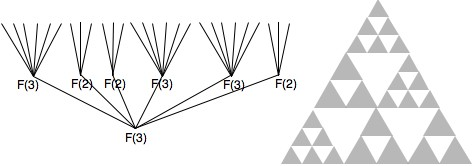
\includegraphics[width=3in]{IFStree.jpg} 
  \caption{Level 2 approximations to an IFS tree and to the associated fractal.  Here   $ \boldsymbol{F} = \{F(2), F(3)\} $  contains the IFSs generating $ SG(2) $ and $ SG(3) $ respectively.  Edges of the tree with a given initial node are enumerated from left to right; they correspond to subcells enumerated anticlockwise from the bottom left corner of the cell corresponding to the given node.}
  \label{IFStree}
\end{figure}

\begin{figure}[htbp] %  figure placement: here, top, bottom, or page
  \centering
  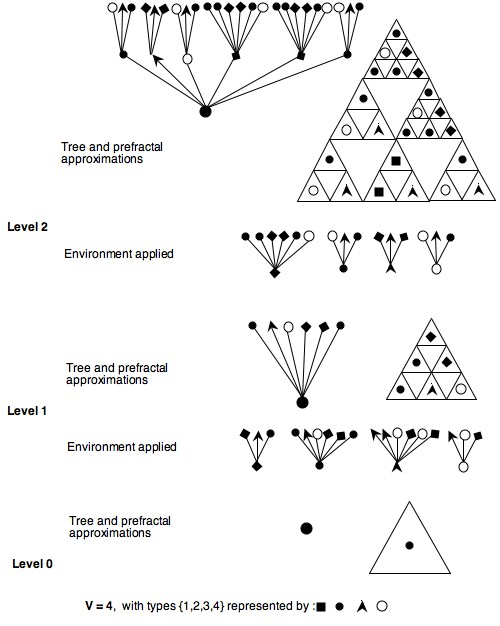
\includegraphics[width=4.5in]{V-var.jpg} 
  \caption{Approximations   to a 4-variable   tree  and the     prefractal approximations to the corresponding 4-variable fractal.  The IFSs are $ F(2) $ and $ F(3) $ generating $ SG(2) $ and $ SG(3) $. The environment at each level is applied to the approximation  at the previous level.   The IFS labels  are not shown  but   are here determined by the branching number.}
  \label{V-var}
\end{figure}





\begin{defn} \label{dfVt}  (See Figure~\ref{V-var})
A  \emph{$ V $-variable (IFS) tree} is an IFS tree $ T $ with a \emph{type} $ \tau  ^{ \boldsymbol{i} } \in \{1,\dots, V \} $ associated to each node $ \boldsymbol{i} $, such that  if two nodes at the \emph{same} level $ k $  have the same type then:
\begin{enumerate}
\item   both nodes have the same branching number and   associated IFS, i.e.
\[ 
|\boldsymbol{i} | = | \boldsymbol{j} | \ \&\ \tau ^{\boldsymbol{i}}= \tau ^{\boldsymbol{j} }
\    \Longrightarrow \ N^ { \boldsymbol{i} } = N^ { \boldsymbol{j} }  \ \& \ F^ { \boldsymbol{i} } = F^ { \boldsymbol{j} } ;
    \]

   \item   comparable successor nodes   have the same type as each other, i.e.
   \[
|\boldsymbol{i} | = | \boldsymbol{j} | \ \&\ \tau ^{\boldsymbol{i}}= \tau ^{\boldsymbol{j} }
\ \&\ 1 \leq p \leq  N^ { \boldsymbol{i} }  \  \Longrightarrow \ 
\tau ^{ \boldsymbol{i}  p } =   \tau ^{ \boldsymbol{j}  p } .
\]
   \end{enumerate} 
The recursive fractal $ K = K(T) $ corresponding to the  $ V $-variable   tree $ T $ is called a \emph{$ V $-variable fractal}.    
   The  \emph{class  of   $ V $-variable trees and class of $ V $-variable fractals} corresponding to $ \boldsymbol{F} $ are denoted by $ \mathcal{T}  ^F_V = \mathcal{T} _  V $ and $ \mathcal{K} ^F_V = \mathcal{K} _  V $ respectively.
     \end{defn}     

\begin{remark} \label{rm1v}
A  1-variable   tree  is essentially the same as an IFS tree  which generates a scale irregular, i.e.\ homogeneous, fractal.

A $ V $-variable   tree  has at most $  V $ distinct IFSs associated to the nodes at each fixed level.
If two nodes at the \emph{same} level  of  a $ V $-variable   tree have the same type then the subtrees rooted at these two nodes are identical, i.e.\
   \[
| \boldsymbol{i} | = | \boldsymbol{j}  |
 \ \&\ \tau ^{\boldsymbol{i}}= \tau ^{\boldsymbol{j} }
 \  \Longrightarrow\  \sigma _{ \boldsymbol{i} } T = \sigma _ { \boldsymbol{j} } T .
\]
In particular there are at most $ V $ distinct subtrees rooted at the \emph{same} level.
\hfill $\square$  \end{remark}  

The following is used in the construction and analysis of $ V $-variable fractals.

\begin{defn} \label{dfenv}  An \emph{environment} $ \mathcal{E}$ assigns to each type $v \in \{1,\dots, V \} $ an  IFS $ F= F_v \in \boldsymbol{F} $ and a sequence of types $( \tau_{v1}, \dots, \tau_{vN_v})$, where $ N_v = |F_v| $.  We write 
\[
\mathcal{E} = (E^{\mathcal{E}}_1,\dots, E^{\mathcal{E}}_V),\quad   E^{\mathcal{E}}_v 
      = (F^{\mathcal{E}}_v,  \tau^{\mathcal{E}}_{v1}, \dots,  \tau^{\mathcal{E}}_{v N_v }). 
\]
\end{defn} 

For the following consider the case $ n=2 $ in Figure~\ref{V-var}.

\begin{constr} 
$ V $-variable   trees are constructed recursively  as follows:
\begin{enumerate}

\item \emph{Stage 0}:  Assign a type $ \tau^\emptyset $ to the root node $ \emptyset $.

\item Assume that by the completion of stages $ 0$  to $  n-1$: 
\begin{enumerate}
\item the tree and all nodes $ \boldsymbol{i} $ with  $ | \boldsymbol{i} | \leq n-1 $ have been constructed,
\item a type $ \tau ^ { \boldsymbol{i} } $ has been assigned if  $ | \boldsymbol{i} | \leq n-1 $, 
\item an IFS $F ^ { \boldsymbol{i} } $ has been assigned if  $ | \boldsymbol{i} | \leq n-2 $, 
\item  the two properties in Definition~\ref{dfVt}  hold if  $ | \boldsymbol{i} | \leq n-2 $.
\end{enumerate}  

\item   \emph{Stage n}:  Choose an environment $ \mathcal{E} $.  We follow the notation of Definition~\ref{dfenv}  and use $ \mathcal{E}  $ in the obvious way to assign an IFS to the level $ n-1 $ nodes, to construct the level $ n $ nodes, and to assign a type to every level $ n $ node.  

More precisely, for each node $ \boldsymbol{i} $ with  $ | \boldsymbol{i} | = n -1 $, if $ v = \tau ^{\boldsymbol{i} } $ is the type already assigned to $ \boldsymbol{i} $, then:
\begin{enumerate}
\item    $ F^{\boldsymbol{i}} := F^{\mathcal{E} }_v$   is the IFS assigned to $ \boldsymbol{i} $, 
\item the branching number $ N^{ \boldsymbol{i} } $ at $ \boldsymbol{i} $ is $ |F^{\boldsymbol{i}}| $,
\item for $ 1\leq j \leq |F^{\boldsymbol{i}}| $ the type $\tau ^{\boldsymbol{i} j } := \tau^{\mathcal{E}}_{vj} $ is the type assigned to the level $ n $  node $ \boldsymbol{i} j $ .
\end{enumerate} 
\end{enumerate} 

It follows by an easy induction that the properties in  Definition~\ref{dfVt} hold at all nodes.
\hfill $\square$  \end{constr} 

\begin{defn} \label{dfneck} The environment $ \mathcal{E} $ in Definition~\ref{dfenv}  is a \emph{neck}  if all $ \tau _{vi} ^{\mathcal{E} } $ are equal.
A \emph{neck  occurs at level $ n $} in the construction of a $ V $-variable   tree if the environment $ \mathcal{E} $ applied at stage $ n $ is a neck environment.
\end{defn} 

\begin{figure}[htbp] %  figure placement: here, top, bottom, or page
   \centering
   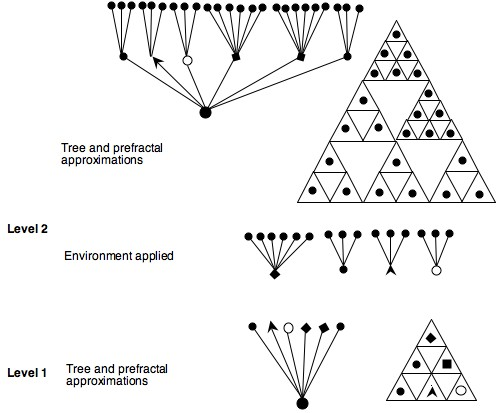
\includegraphics[width=4in]{neck.jpg} 
   \caption{Compare with Figure~\ref{V-var}, except that now a neck occurs at level 2.  All subtrees rooted at this level will be the same, although they have not yet been constructed.  All 2-complexes will be the same up to scaling by   factors determined by the construction up to this level.}
   \label{figneck}
\end{figure}

If a neck occurs at level $ n $  then the type assigned to every node at that level is the same. See Figure~\ref{figneck}.  It follows from 
Remark~\ref{rm1v}  that all subtrees rooted at level $ n $ will be the same. Note that the subtrees are only constructed at later stages, and even  the common  value of the IFS at each level $ n $ node is not determined until stage $ n+1 $.  

There is however no restriction on the IFSs occurring in a neck environment $ \mathcal{E} $. For a level $ n $ neck  these IFSs are applied at level $ n-1 $.  


Because there is an upper bound on the number of functions $ N^F $ in any IFS $ F \in \boldsymbol{F} $, there is only a finite number of type choices to be made in selecting an environment. It follows that necks   occur infinitely often almost surely with respect to the probability$ P_V $ defined in Definition~\ref{dfpv2}.  The sequence of neck levels in the construction of a $ V $-variable tree or neck is denoted by
\[
0= n(0) < n(1) < \dots < n(i) < \cdots .
\]



\begin{defn} \label{dfpv} Fix a probability distribution $ P $ on $ \boldsymbol{F} $.  This induces a \emph{probability distribution $ P_V $ on the set of environments} as follows. Choose the IFSs $ F^{\mathcal{E} } _v $ for $ v \in \{1,\dots,V\} $ in an iid manner according to $ P $.   Choose types $ \tau ^{\mathcal{E}} _{vj} $ for $ 1 \leq j \leq | F^{\mathcal{E} } _v | $   in an iid manner according to the uniform distribution on $ \{1,\dots, V \} $ and otherwise independently of the  $ F^{\mathcal{E} } _v$.
\end{defn}

\begin{defn}  \label{dfpv2}
The \emph{probability distribution on the set $ \mathcal{T}_V $} of $ V $-variable   trees is obtained by choosing $ \tau ^\emptyset $ according to the uniform distribution and independently choosing the environments at each stage in an iid manner according to $ P_V $. This probability distribution on $ V $-variable  trees induces a \emph{probability distribution on the set $ \mathcal{K} _V $} of $ V $-variable fractals.  Both the distributions on trees and on fractals are also denoted by $ P_V $.

The $ \sigma $-algebra of measurable subfamilies of $ \mathcal{K}_V $ is the Borel $ \sigma $-algebra induced by the 
Hausdorff metric on nonempty compact subsets of $ \mathbb{R}^d $.  For $ \mathcal{T}_V $ one uses any of the standard tree metrics.

\emph{Random $ V$-variable   trees} and \emph{random $ V $-variable fractals} are random labelled trees and random compact subsets of $ \mathbb{R}^d  $ respectively   with the distribution $ P_V$. We write $ T $ or $ T^ \omega $, and $ K $ or  $ K^ \omega $, respectively.

It will normally be convenient to identify the sample space for our random quantities (fractals, trees, etc) with the set of $ V $-variable IFS trees.  For example,  $ \sigma_{ \boldsymbol{i} } \omega $ is just the transfer operator   defined in Notation~\ref{notn1} for a tree $ T $. 
\end{defn}








%%%%%%%%%%%%%%%%%%%%%%%%%%%%%%%%%%%%
\clearpage \begin{thebibliography}{9} 

   \bib{BHS}{article}{
    author={Barnsley, M. F.},
    author={Hutchinson, John E.},
    author={Stenflo, {\"O}rjan},
    title={V-variable Fractals: Dimension results},
   note={Forum Mathematicum, to appear, 2010},   
%   date={2009},   
}


\bib{Sce1}{thesis}{
   author={Scealy, Bob},
   title={V-variable fractals and interpolation},
  note={draft Version, 7 September}, 
  date={2007}
     }

\bib{Sce2}{thesis}{
   author={Scealy, Bob},
   title={V-variable fractals and interpolation},
%  note={Preliminary Version, 7 September 2007}, 
  date={2008}
     }

\end{thebibliography} 
\end{document} 






\begin{figure}[htbp] %  figure placement: here, top, bottom, or page
   \centering
   
\includegraphics[width=5in]{V-vargen1T.jpg} \\ \mbox{} \\
   
\includegraphics[width=1in]{V-vargen0.jpg} \hspace{5cm}
   
\includegraphics[width=1in]{V-vargen1.jpg} 
   \caption{Initial cell of type green.  The 4 transformation rules at time 1 (only the second is relevant).  The resulting organism at time 1.}
   \label{V-vargen1}
\end{figure}




\begin{figure}[htbp] %  figure placement: here, top, bottom, or page
   \centering
   
\includegraphics[width=5in]{V-vargen2T.jpg} \\ \mbox{} \\
   
\includegraphics[width=1in]{V-vargen1.jpg}  \hspace{4cm}
    
\includegraphics[width=1in]{V-vargen2.jpg} 
   \caption{The organism at time 1. The transformation rules at time 2. The resulting organism at time 2.}
   \label{V-vargen2}
\end{figure}
 










\begin{figure}[htbp] %  figure placement: here, top, bottom, or page
   \centering
   
\includegraphics[width=5in]{V-vargen3T.jpg} \\ \mbox{} \\
   
\includegraphics[width=2.2in, height=2in]{V-vargen2.jpg}  \hspace{2cm}
    
\includegraphics[width=2.2in, height=2in]{V-vargen3.jpg} 
   \caption{the organism at time 2. The transformation rules at time 3.  The resulting organism at time 3.}
   \label{V-vargen3}
\end{figure}
 
%%%%%%%%%%%%%%%%%%%%%%%%%%%%%%%%%%%%%%%%%%%


%%%%%%%%%%%%%%%%%%%%%%%%%%%%%%%%%%%%%%%%%
%%%%%%%%%%%%%%%%%%%%%%%%%%%%%%%%%%%%%%%%%
\newpage \subsection{Backward Process}   See Figure~\ref{g3sg}.



\begin{figure}[htbp] %  figure placement: here, top, bottom, or page
   \centering
   
\includegraphics[width=3.5in]{V-cat.jpg} 
   \caption{Level 1, 2 and 3 prefractals in the generation process  for a 3-variable Sierpinski Gasket.
   On the left of the large arrows are indicated the IFSs used to transform the red, blue and green cells at the previous level.  The partitions of the new cells into red, blue and green are also indicated.}
   \label{g3sg}
\end{figure}

\begin{figure}[htbp] %  figure placement: here, top, bottom, or page
   \centering
   
\includegraphics[width=3.5in]{V-cat2.jpg} 
   \caption{Box representation of the same example.  The red, blue and green boxes show the IFSs used to transform the red, blue and green cells at the previous level.  The partitions of the new cells into red, blue and green are also indicated.}
   \label{g3sg2}
\end{figure}


Given data consists of a family $ \mathcal{F} $ of IFS's $ \{ F^ \lambda = (\psi^  \lambda _1,\dots, \psi^ \lambda _{M_\lambda });   \lambda \in \Lambda  \}$,    a natural number  $ V \geq 1 $ and a probability distribution $ P $ on $ \Lambda $.

For the example in Figure~\ref{g3sg}, $ \mathcal{F} $ contains the two IFSs
$F^2= (\psi^2_1,\psi^2_2,\psi^2_3)  $ and $F^3= (\psi^3_1,\dots,\psi^3_6)  $ generating $ SG(2) $ and $ SG(3) $ respectively.
The corresponding probability distribution is given by  $ P(2) = p $ and $ P(3) = q $.

\medskip Each realisation%
\footnote{Not just a.e.\ realisation.}
$ \omega $ of the generation process  produces 
 a sequence of level $ n $ prefractals $ G^n = G^n(\omega) $ whose limit $ G = G(\omega) $ is a $ V  $-variable fractal.
 The probability $ P $ is not required for this.

The probability distribution  $ P $  gives a natural probability distribution on the generation process such that $ \omega \mapsto G(\omega) $ is a random $ V $-variable fractal with a natural probability distribution.


\medskip
It is helpful to assume each $ F^ \lambda $ is pcf with a common base set  $ V^{(0)} $.  In Figure~\ref{g3sg}, $ V^{(0)} $ is interpreted as the set of vertices of the standard equilateral triangle in~$ \mathbb{R}^2 $.  

Alternatively, assume that there is a compact subset $ T $ independent of $ \lambda $ such that $ F^ \lambda (T) \subset T $ for each $ \lambda $.  In Figure~\ref{g3sg}, $ T $ is the closed convex hull of the standard equilateral triangle in~$ \mathbb{R}^2 $. 

\medskip
The case $ V=1 $  corresponds to the homogeneous random fractal case.
The case $ V $ large approximates the random recursive case.  

%%%%%%%%%%%%%%%%%%%%%%%%%%
\subsubsection{Summary}  (The process can be applied with or without using the probability distribution $ P $.  The probabilistic aspects of the construction are in parentheses.)

In the first step an IFS is chosen (via $ P $), a level 1 prefractal is obtained by applying this IFS to the level 0 prefractal common to all the IFSs, and the resulting 1-cells are partitioned   into   $ V $ equivalence classes (each 1-cell independently according to the uniform distribution on $\{ 1,\dots, V \}$).

After  step $ n $ for $ n\geq 1$, one has obtained a level $ n $ prefractal together with a partition of its $ n $-cells  into $ V $ equivalence classes. 
In the subsequent step $ n + 1 $ one selects an IFS for each of these $ V $ equivalence classes of $ n $-cells (independently according to $ P $), applies this \emph{same} IFS to \emph{each} $ n $-cell in the equivalence class, and partitions the resulting $ n+1 $-cells into  $ V $ equivalence classes (independently for the $ n+1 $-cells corresponding to a fixed $ n$-cell) and in the \emph{``same''} way for the $ n+1 $-cell ``children'' of each $ n $-cell in the same equivalence class. 


%%%%%%%%%%%%%%%%%%%%%%%%%%%

\subsubsection{Details} 
\begin{enumerate}
\item The level 1 prefractal is obtained by applying $ F^\lambda $ to $  V^{(0)} $ or to $ T $, and then partitioning the resulting 1-cells into $ V $  possibly empty equivalence classes.  

(In the probabilistic case $ F^\lambda $ is chosen via $ P $.  The equivalence class  for each 1-cell is then chosen independently according to the uniform distribution.)


In Figure~\ref{g3sg}  see the bottom row, where the IFS $ F^2 $ is applied and equivalence classes of 1-cells are represented by   red, blue and green (the latter class is empty in the example).

\item The level 2 prefractal is obtained by applying an  $ F^\lambda $ to each 1-cell in the level 1 prefractal and partitioning the resulting 2-cells into $ V $  possibly empty equivalence classes.  The same IFS is applied to equivalent 1-cells and the same partition is then applied to the resulting 2-cells.

(In the probabilistic case the IFS for each equivalence class  is chosen independently via $ P $.  For a fixed 1-cell the equivalence class  for each resulting  2-cell is chosen independently  according to the uniform distribution.  The ``same'' partition is used for every 1-cell in the same equivalence class, but different equivalence classes are treated independently.)

In Figure~\ref{g3sg}  the non empty classes of 1-cells correspond to red and blue, the corresponding IFS and partitions are indicated on the left of the middle row of figures, and the resulting  level 2 prefractal with its partition of 2-cells is shown on the right.

\item  The level 3 prefractal is obtained by applying some  $ F^\lambda $ to each 2-cell in the level 2 prefractal and partitioning the resulting 3-cells into $ V $  possibly empty equivalence classes.  The same IFS is applied to equivalent 2-cells and the same partition is then applied to the resulting 3-cells.

(In the probabilistic case the IFS for each equivalence class  is chosen independently via $ P $.  For a fixed 2-cell the equivalence classes for each resulting  3-cell is chosen independently   according to the uniform distribution. The ``same'' partition is used for every 2-cell in the same equivalence class, but different equivalence classes are treated independently.)

In Figure~\ref{g3sg} the  equivalence classes of 1-cells again correspond to red, blue and green; the corresponding IFS and partitions are indicated on the left of the top row of figures, and the resulting  level 3 prefractal with its partition of 3-cells is shown on the right.
\end{enumerate} 
 

%%%%%%%%%%%%%%%%%%%%%%%%%%%%%%%%%%%%%%%%%
\subsection{Forward Process}  


